\chapter{Internal Application Structure} \label{sec:coreframework}

The firmware is built around a \textit{core framework} which provides services to units, such as the settings storage, resource allocation, message delivery, and periodic updates. In this chapter, we will focus on the structure of this framework and the services provided by it.

\section{Internal Structure Block Diagram}

The data flows and other internal logic of the firmware are depicted in \cref{fig:gexinternal}, with more explanation following in this chapter. The interchangeable role of the three communication interfaces can be clearly seen in the diagram, as well as the central role of the message queue, which decouples interrupts from the processing thread.

\begin{figure}[h]
	\centering
	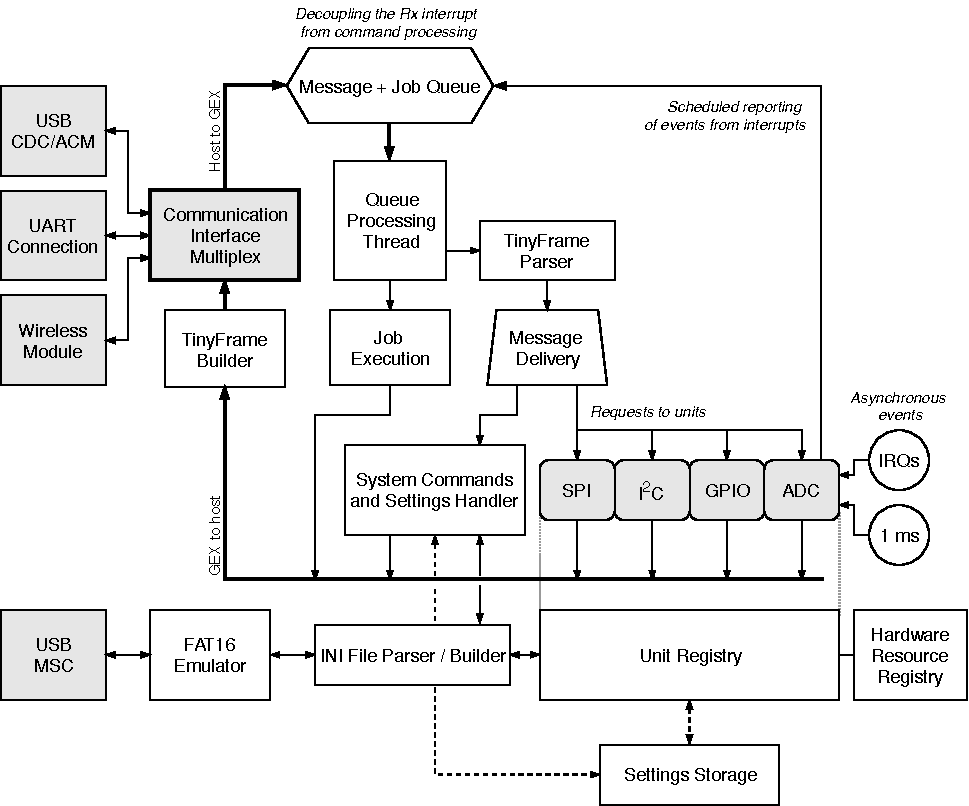
\includegraphics[width=\textwidth] {img/gex-internal.pdf}
	\caption{\label{fig:gexinternal}Block diagram showing the internal logic in the GEX firmware}
\end{figure}

The core framework forms the skeleton of the firmware and usually does not need any changes when new user-facing features are added. When the firmware is ported to a different STM32 microcontroller, the framework is not difficult to adjust and the whole process can be accomplished in a few hours. The porting of units to a different platforms is significantly more challenging.

\noindent
The framework provides the following services to units:

\begin{itemize}
	\item Hardware resource allocation (\cref{sec:res_allocation})
	\item Settings storage and loading (\cref{sec:settings_storage})
	\item Unit life cycle management (\cref{sec:units_function})
	\item Message sending and delivery (\cref{sec:message_passing})
	\item Interrupt routing (\cref{sec:irq_routing})
\end{itemize}

\section{Unit Life Cycle and Internal Structure} \label{sec:units_function}

GEX's user-facing functions, units, are implemented in \textit{unit drivers}. Those are independent modules in the firmware that the user can enable and configure, in one or more instances. In practice, we are limited by hardware constraints: i.e., there may be only one \gls{ADC} peripheral, or two \gls{SPI} ports. The assignment of those hardware resources to units is handled by the \textit{resource registry} (\cref{sec:res_allocation}).



Each unit is identified by a name and a \textit{callsign}, which is a number that serves as an address for message delivery. A unit is internally stored as a data object with the following structure:

\begin{itemize}[itemsep=0pt]
	\item Name
	\item Callsign (one byte)
	\item Configuration parameters loaded from the unit settings
	\item State variables updated at run-time by user commands or internal functions
	\item A reference to the unit driver
\end{itemize}

The unit driver handles commands sent from the host \gls{PC}, initializes and de-initializes the unit based on its settings, and implements other aspects of its function, such as periodic updates and interrupt handling. 

When the units configuration file is modified, all units are de-initialized and removed. The binary settings are then updated based on the new values, verifying that the requested resources are available, and the units that can be enabled are subsequently initialized and made available to the user.

\section{Resource Allocation} \label{sec:res_allocation}

\begin{figure}[h]
	\centering
	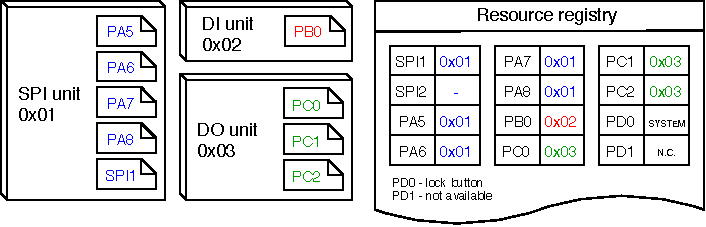
\includegraphics[scale=1] {img/resource-repository.pdf}
	\caption{\label{fig:resource_repository}An example allocation in the resource registry}
\end{figure}

The microcontroller provides a number of hardware resources that require exclusive access: GPIO pins, peripheral blocks (\gls{SPI}, \gls{I2C}, \gls{UART}\textellipsis), and \gls{DMA} channels. If two units tried to control the same pin, the results would be unpredictable; similarly, the output of a multiply-accessed serial port could become a useless mix of the different data streams.

To prevent multiple access, the firmware includes a \textit{resource registry} (\cref{fig:resource_repository}). Each individual resource is represented by a field in a resource table together with its owner's callsign. Initially all resources are free, except for those not available on the particular platform (e.g., a \gls{GPIO} pin PD1 may be disabled if not present on the microcontroller's package).

The resources used by the core framework are taken by a virtual unit \verb|SYSTEM| on start-up to prevent conflicts with the user's units. This is the case of the status \gls{LED}, the Lock button, \gls{USB} pins, the communication \gls{UART}, the pins and an \gls{SPI} peripheral connecting the wireless module, pins used for the crystal oscillator, and the timer/counter which provides the system timebase.


\section{Settings Storage} \label{sec:settings_storage}

\begin{figure}[h]
	\centering
	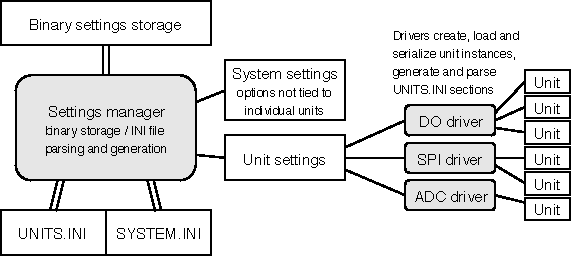
\includegraphics[scale=1.2] {img/settings-storage.pdf}
	\caption{\label{fig:settings_storage}Structure of the settings subsystem}
\end{figure}

The system and unit settings are written, in a binary form, into designated pages of the microcontroller's Flash memory. The unit settings serialization and parsing is implemented by the respective unit drivers.

As the settings persist after a firmware update, it is important to maintain backward compatibility. This is achieved by prefixing the settings block of each unit with a version number. When the settings are loaded by a new version of the firmware, it first checks the version and decides whether to use the old or new format. When the settings are next changed, the new format will be used.

\iffalse 
The INI files, which can be edited through the communication \gls{API} or using a text editor through the virtual mass storage, are parsed and generated on demand and are never stored in the Flash or \gls{RAM}, other than in short temporary buffers. The INI parser processes the byte stream on-the-fly as it is received, and a similar method is used to build a INI file from the configured units and system settings. \fi % said elsewhere


\section{Message Passing} \label{sec:message_passing}

One of the key functions of the core framework is to deliver messages from the host \gls{PC} to the right units. The \textit{TinyFrame} protocol is used, described in detail in \cref{sec:tinyframe}; it is represented by the blocks ``TinyFrame Parser'' and ``TinyFrame Builder'' in \cref{fig:gex_internal}.

Two groups of messages exist: \textit{system messages} and \textit{unit messages}. System messages can, for instance, access the INI files, or request a list of available units. Unit messages are addressed to a particular unit, and their payload format is defined by the unit's driver. An incoming message is inspected and delivered to the appropriate recipient, or responded to with an error message.

In addition to message delivery, the core framework also provides event reporting. Events are messages generated by units and sent to the host to notify it about asynchronous events.

This high-level functionality resides above the framing protocol, which will be described in \cref{sec:tinyframe}. The message format is shown in \cref{sec:unit_requests_reports}.


\section{Interrupt Routing} \label{sec:irq_routing}

Interrupts are an important part of almost any embedded application. They provide a way to rapidly react to asynchronous external or internal events, temporarily leaving the main program, jumping to an interrupt handler routine, and then returning back after the event is handled. Interrupts are also the way FreeRTOS implements multitasking without a multi-core processor.

In \arm Cortex-M0 the interrupt handlers table, defining which routine is called for which interrupt, is stored in the program memory and cannot be changed at run-time. This is a complication for the modular structure of GEX where different unit drivers may use the same peripheral, and we would want to dynamically assign the interrupt handlers based on the active configuration. 


Let us have a look at a sample interrupt handler, in this case serving four different \gls{DMA} channels, as is common in STM32 microcontrollers:

\begin{minted}{c}
void DMA1_Channel4_5_6_7_IRQHandler(void)
{
    if (LL_DMA_IsActiveFlag_GI4(DMA1)) { /* handle DMA1 channel 4 */ }
    if (LL_DMA_IsActiveFlag_GI5(DMA1)) { /* handle DMA1 channel 5 */ }
    if (LL_DMA_IsActiveFlag_GI6(DMA1)) { /* handle DMA1 channel 6 */ }
    if (LL_DMA_IsActiveFlag_GI7(DMA1)) { /* handle DMA1 channel 7 */ }
}
\end{minted}

It is evident that multiple units might need to use the same handler, even at the same time, since each \gls{DMA} channel is configured, and works, independently. GEX implements a redirection scheme to accomplish such interrupt sharing: All interrupt handlers are defined in one place, accompanied by a table of function pointers. When a unit driver wants to register an interrupt handler, it stores a pointer to it in this redirection table. Then, once an interrupt is invoked, the common handler checks the corresponding entry in the table and calls the referenced routine, if any. Conversely, when a unit driver de-initializes a unit, it removes all interrupt handlers it used, freeing the redirection table slots for other use.

\section{FreeRTOS Synchronization Objects Usage} \label{sec:rtos_in_gex}

The firmware is built around FreeRTOS (\cref{sec:freertos}) and a number of its synchronization objects and patterns are used to make its operation more robust.

\subsection{Message and Job Queue}

The message and job queue, seen in \cref{fig:gexinternal}, is used to decouple asynchronous interrupts from message transmission. All three communication interfaces use interrupts for the asynchronous handling of incoming messages. The same interrupt handler receives an event after a transmission was completed. The queue ensures that messages can be received during the transmission of a large response that demands the use of multiple transmissions.

The ``transmission complete'' interrupt signals this fact to the message processing task using a binary semaphore. The semaphore is released in the \gls{ISR} and taken when a new block of data is to be transmitted. If more data needs to be transmitted, the queue task waits for the semaphore and enters a Blocked state until the semaphore becomes available again.

Two mutexes are used in the firmware: one that guards access to TinyFrame until the previous message was fully transmitted, and one to guard a shared memory buffer (reused in several different places to save memory and avoid its re-allocation). The hardware resource registry (explained in \cref{sec:res_allocation}) does not need mutexes for individual resources, as concurrent access to those fields can never happen; resources are always taken or released sequentially by the same task.


\section{Source Code Layout}

\begin{wrapfigure}[22]{r}{0.4\textwidth}
	\scriptsize\vspace{-3em}
	\begin{verbatim}
	├── build
	│   ├── firmware.bin
	│   └── firmware.dfu
	├── Drivers
	│   ├── CMSIS
	│   │   └── Device / ST / STM32F0xx
	│   └── STM32F0xx_HAL_Driver
	├── Middlewares / Third_Party / FreeRTOS
	├── Src
	│   └── main.c
	├── User
	│   ├── USB / STM32_USB_Device_Library
	│   │   ├── Class
	│   │   │   ├── CDC
	│   │   │   ├── MSC
	│   │   │   └── MSC_CDC
	│   │   └── Core
	│   ├── platform
	│   │   ├── plat_compat.h
	│   │   └── platform.c
	│   ├── units
	│   │   ├── adc
	│   │   ├── digital_out
	│   │   ...
	│   ├── FreeRTOSConfig.h
	│   └── gex.mk
	└── Makefile
	\end{verbatim}
	\vspace{-1em}
	\caption{\label{fig:repo_structure} The general structure of the source code repository}
\end{wrapfigure}

Looking at the GEX source code repository (\cref{fig:repo_structure}), at the root we'll find the device specific driver libraries and support files provided by ST Microelectronics, the FreeRTOS middleware, and a folder called \verb|User| containing the GEX application code. This division is useful when porting the firmware to a different microcontroller, as the GEX folder is mostly platform-independent and can be simply copied (of course, adjustments are needed to accompany different hardware peripheral versions etc.). The GEX core framework consists of everything in the \verb|User| folder, excluding the \verb|units| directory in which the individual units are implemented. Each unit driver must be registered in the file \verb|platform.c| to be available for the user to select. The file \verb|plat_compat.h| includes platform-specific headers and macros, defining parameters such as pin assignments or the clock speed.

The \gls{USB} Device library, which had to be modified to support a composite class, is stored inside the \verb|User| folder too, as it is compatible with all STM32 microcontrollers that support \gls{USB}.











